%amsart class
\documentclass[a4paper, 10pt, reqno]{amsart}

%Packages
\usepackage[utf8]{inputenc}
\usepackage[english]{babel}
\usepackage{graphics}
\usepackage{physics}
\usepackage{listings}
\usepackage{hyperref}
\usepackage{blindtext}
\usepackage{xcolor}
\usepackage[position=top]{subfig}
\usepackage{pgf}
\usepackage{tikz}
\usepackage{tikzscale}
\usepackage{pgfplots}
\usepackage{placeins}
\usepackage{parskip}

\hypersetup{colorlinks=true, linkcolor=black, citecolor=black,
urlcolor=blue}
%\hypersetup{hidelinks}

\pgfplotsset{compat=1.5}
\newlength\figureheight
\newlength\figurewidth
\setlength\figurewidth{0.98\textwidth}
\setlength\figureheight{0.75\figurewidth}

\usepackage{etoolbox}
\makeatletter
\patchcmd{\@maketitle}
  {\ifx\@empty\@dedicatory}
  {\ifx\@empty\@date \else {\vskip3ex
  \centering\footnotesize\@date\par\vskip1ex}\fi
   \ifx\@empty\@dedicatory}
  {}{}
\patchcmd{\@adminfootnotes}
  {\ifx\@empty\@date\else \@footnotetext{\@setdate}\fi}
  {}{}{}
\makeatother

%Custom colors
\definecolor{code}{rgb}{0.9, 0.17, 0.31}
\definecolor{coolgrey}{rgb}{0.55, 0.57, 0.67}
\definecolor{cyan(process)}{rgb}{0.0, 0.72, 0.92}
\definecolor{lightwhite}{rgb}{0.9647058823529412, 0.9647058823529412, 0.9647058823529412}
\definecolor{royalblue}{rgb}{0.25, 0.41, 0.88}
\definecolor{mediumseagreen}{rgb}{0.24, 0.7, 0.44}
%listing customization
\lstset{ %
  backgroundcolor=\color{lightwhite},
  basicstyle=\ttfamily\footnotesize,        % the size of the fonts that are used for the code
  breakatwhitespace=true,         % sets if automatic breaks should only happen at whitespace
  breaklines=true,                 % sets automatic line breaking
  captionpos=b,                    % sets the caption-position to bottom
  commentstyle=\color{mediumseagreen},    % comment style
  deletekeywords={...},            % if you want to delete keywords from the given language
  escapeinside={\%*}{*)},          % if you want to add LaTeX within your code
  extendedchars=true,              % lets you use non-ASCII characters; for 8-bits encodings only, does not work with UTF-8
  frame=single,	                   % adds a frame around the code
  keepspaces=true,                 % keeps spaces in text, useful for keeping indentation of code (possibly needs columns=flexible)
  keywordstyle=\color{code},       % keyword style
  language=[90]Fortran,                 % the language of the code
  otherkeywords={...},           % if you want to add more keywords to the set
  emph={get_H_p, spline, exp, abs, sqrt},
  emphstyle={\color{royalblue}},
  rulecolor=\color{white},         % if not set, the frame-color may be changed on line-breaks within not-black text (e.g. comments (green here))
  numbers=left,
  showspaces=false,                % show spaces everywhere adding particular underscores; it overrides 'showstringspaces'
  showstringspaces=false,          % underline spaces within strings only
  showtabs=false,                  % show tabs within strings adding particular underscores
  stepnumber=1,                    % the step between two line-numbers. If it's 1, each line will be numbered
  tabsize=3,	                   % sets default tabsize to 2 spaces
}

%Frontpage stuff
\title[Milestone 1]{\Large{Milestone 1: The background evolution of the universe} \\
\normalsize{FYS5220 - Cosmology 2}}

\author[San]{Metin San}

\date{\today}



%Begining document
\begin{document}

\maketitle
\begin{center}
   \vspace*{-0.6cm} \textsc{\url{https://github.com/MetinSa/AST5220}}
\end{center}

\begin{abstract}
    We set up the cosmological grids for the scale factor $a$, the
    redshift $z$ and the parameter $x = \log a$. These are then applied
    to compute the time evolution of the background density and the
    Hubble parameter. Finally we compute the conformal time $\eta$ and
    spline it to interpolate between the grid points in order to
    achieve a better accuracy at .
\end{abstract}

\section{Introduction}
The long-term goal of the numerical aspect of this course is to
simulate the Cosmic Microwave Background (CMB); mainly through the
calculation of the power spectrum. This will be a gradual process, with
this report constituting the first milestone. The goals of milestone 1
will be to study the expansion history of the universe, as well as
looking at how the uniform background densities of the various matter
and energy components evolve. We will do so by exploring the Hubble
parameter along with the conformal time.

The code used for the numerical calculations is written in FORTRAN 90
and is based on the provided skeleton code. The analysis of the data is
done using Python. All source codes and tools used to produce the
results and figures can be found on my Github by following the link
below the author name on the front page.

The report will consist of a theory section where we introduce and
motivate the assumptions and theory used to make our calculations. What
follows is the result section where we present and discuss our results.
We then conclude the report with a small section where we reflect back
on the work done.

\section{Theory}
We begin by introducing some cosmological concepts which are necessary
in order to compute and study the expansion history of the Universe. We
start by assuming a flat universe $(k=0)$ described by the
Friedmann-Robertson-Walker metric in which the line element (in polar
coordinates) is given by
\begin{equation}\label{eq: ds}
    ds^2 = -c^2 dt^2 + a^2(t) \left( dr^2 + r^2(d\theta^2 + \sin^2
    \theta d\phi^2) \right),
\end{equation}
where $a(t)$ is the scale factor. The scale factor is connected to the
redshift through the relation
\begin{equation}\label{eq: redshift}
    1 + z = \frac{a(t_0)}{a(t)},
\end{equation}
where $a(t_0) = 1$ is the scale factor today. We will then define the
parameter $x$
\begin{equation}\label{eq: x}
    x \equiv \ln a.
\end{equation}
This parameter makes it easier to work with the quantities we are about
to compute as we will mainly work with phenomena that varies strongly
over wide time ranges. 

We proceed by considering a photon which propagates in this Universe.
The line element for the photon is equal to zero, meaning that equation
\eqref{eq: ds} can be written on the following form in Cartesian
coordinates
\begin{equation}\label{eq: dxdt}
    \frac{dx}{dt} = \frac{c}{a(t)}.
\end{equation}
We then define the conformal time which is given by integrating
equation \eqref{eq: dxdt}
\begin{equation}\label{eq: eta}
    \eta(t) \equiv x = \int_0^{t} \frac{c dt}{a(t)}.
\end{equation}
The conformal time acts as the particle horizon and tells us the
maximum distance from which particles could have traveled to an
observer in the age of the Universe. This is a useful quantity for our
purposes as it relates the expansion of the Universe to a time. The
line element can be expressed in terms of the conformal time
\begin{equation}\label{eq: ds_eta}
    ds^2 = a^2(t) \left( -d^2\eta + dr^2 + r^2(d\theta^2 + sin^2\theta
    d\phi^2) \right).
\end{equation}
In order to numerically compute the conformal time, we write it on the
differential form
\begin{equation}\label{eq: detadt}
    \frac{d\eta}{dt} = \frac{c}{a}.
\end{equation}
We can then use the chain-rule to rewrite \eqref{eq: detadt} to the
following form
\begin{equation}\label{eq: detada}
    \frac{d \eta}{da} = \frac{c}{a^2 H} = \frac{c}{a \mathcal{H}},
\end{equation}
where the $H$ is the Hubble parameter defined as $H \equiv \Dot{a}/a$,
and $\mathcal{H} \equiv aH$. This allows us to compute the conformal
time as soon as we know how the scale factor evolves. The chain-rule
can further be applied to rewrite \eqref{eq: detada} in terms of the
variable $x$ from definition \eqref{eq: x} to simplify our
calculations, giving us
\begin{equation}\label{eq: detadx}
    \frac{d \eta}{dx} = \frac{c}{\mathcal{H}}.
\end{equation}

The observable associated with the expansion of the Universe is the
Hubble parameter which can be defined through the Friedmann equations
as
\begin{equation}\label{eq: Hubble}
    H = H_0 \sqrt{(\Omega_b + \Omega_m)a^{-3} + (\Omega_r +
    \Omega_\nu)a^{-4} +\Omega_\Lambda}.
\end{equation}
Here $H_0$ is the Hubble parameter today, and $\Omega_b$, $\Omega_m$,
$\Omega_r$, $\Omega_\nu$ and $\Omega_\Lambda$ are the relative
densities of the baryonic matter, dark matter, radiation, neutrinoes
and dark energy today, respectively. We will assume the neutrino
density to be 0 through out all milestones. 

These density fractions are given through each components individual
energy density as $\Omega_i = \rho_i /\rho_c$, where $i =
m,b,r,\nu,\Lambda$ denotes the different species, and $\rho_c$ is the
critical density given as $\rho_c = 3H^2/8\pi G$. The Friedmann
equations also provide a description of how each component evolves with
time through the expanding Universe, which are
\begin{align}\label{eq: dens}
    \rho_m &= \rho_{m,0} a^{-3}\\ 
    \rho_b &= \rho_{b,0} a^{-3}\\
    \rho_r &= \rho_{r,0} a^{-4}\\
    \rho_\nu &= \rho_{\nu,0} a^{-4}\\
    \rho_\Lambda &= \rho_{\Lambda,0},
\end{align}
where the subscript $0$ indicate today's values.

\section{Implementation}

The implementation for this milestone mainly consist of completing the
provided \textbf{time\_mod.f90} module. We will now briefly discuss the
structure of the code in addition to the completed methods and
algorithms.

The code begins by initializing the different variables, parameters,
and constants we are to work with. What follows is the allocation of
arrays for the different quantities of interest. These include the
scale factor $a$, the redshift $z$, the parameter $x$ and the conformal
time $\eta$, along with arrays associated to each of the density
components $\rho_i$. The grids for $a$, $x$ and $z$ are then filled in
a linear manner using the specified initial and end conditions ($z \in
[0, 1630]$). We proceed by setting up a second, independent $x$-grid
for the conformal time using the initial condition $a_\text{init} =
10^{-10}$, and the scale factor today, $a_0 = 1$ as the end condition.

With these grids in place, we are able to calculate the time evolution
of the different density species in the Universe through equations
(\ref{eq: dens} - 15). We can also compute the Hubble parameter through
equation \eqref{eq: Hubble} using $H_0$ and $\Omega_i$ parameters found
in the \textbf{params.f90} file. This is done in the lower section of
the code as a seperate function \textit{get\_H(x)} which returns the
$H$ for a given $x$. Similarely we have two additional functions
\textit{get\_H\_p(x)} and \textit{get\_dH\_p(x)} which returns
$\mathcal{H}$ and its derivative $d\mathcal{H}$.

The next part of the code computes the conformal time $\eta$. In order
to do so we need to solve equation \eqref{eq: detadx}. This is
integrated with the use of the program \textbf{ode\_solver.f90}. The
calculation does however require an initial condition for $\eta$. We
find this by considering equation \eqref{eq: detada}. This equation can
be solved for eta
\begin{equation}
    \eta(a) = \int_0^a \frac{c \, da}{a^2 H(a)}.
\end{equation}
We are only interested in the value for $a = a_\text{init}$, meaning
that the expression is reduced to
\begin{equation}\label{eq: eta_init}
    \eta(a_\text{init}) = \frac{c} {a_\text{init} H(a_\text{init})}.
\end{equation}
We know that the Universe was radiation dominated at early times
meaning that the Hubble parameter can be written as $H = H_0
\sqrt{\Omega_r a^{-4}}$. Inserting this this into \eqref{eq: eta_init},
we find the follow initial condition for the conformal time
\begin{equation}
    \eta(a_\text{init}) = \frac{c a_\text{init}}{H_0 \Omega_r^{1/2}}.
\end{equation}
We proceed by computing a spline through the resulting $\eta$ data
using the provided program \textbf{spline\_1D\_mod}. This helps us
resolve the $\eta$ values between the grid points of interest, and will
come in handy in future calculations.

\section{Results}

\begin{figure}
    \centering
    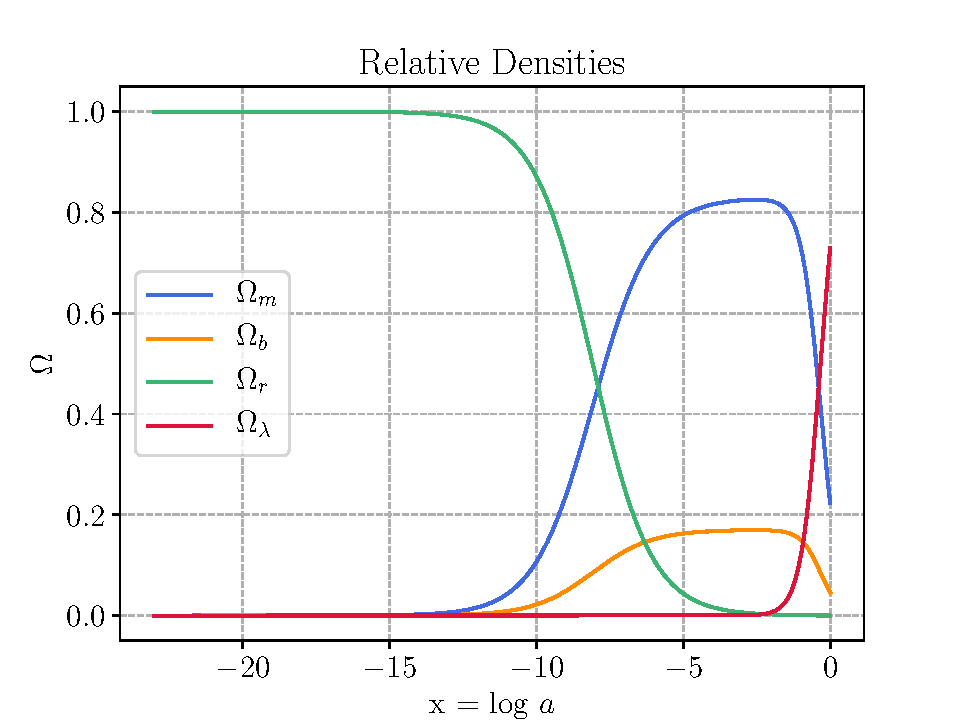
\includegraphics[width = 0.9\textwidth]{densities.pdf}
    \caption{The evolution of the different fractional densities as a
    function of $x$.}
    \label{fig: dens}
\end{figure}

The results of the fractional density evolution calculation is seen in
figure \ref{fig: dens}. As expected, we see that the universe starts of
in an era dominated by $\Omega_r$, the radiation. The dark matter,
$\Omega_m$ overtakes the radiation at $x \approx 8$ and continues to
dominate the universe until around $x \approx 1 $ at which the dark
energy $\Omega_\Lambda$ takes over. The baryons follow the same
behavior as the dark matter as expected since they both scale with
$a^{-3}$ with a lower overall amplitude.

The results of the Hubble parameter calculation can be seen in figures
\ref{fig: H_x} and \ref{fig: H_z} where we have plotted the results
both as functions of the parameter $x$ and the redshift $z$. Both
curves follow the same behaviour. It should be noted that the the
$z$-axis in figure \ref{fig: H_z} has been flipped in order to resemble
figure \ref{fig: H_x}.

\begin{figure}
    \centering
    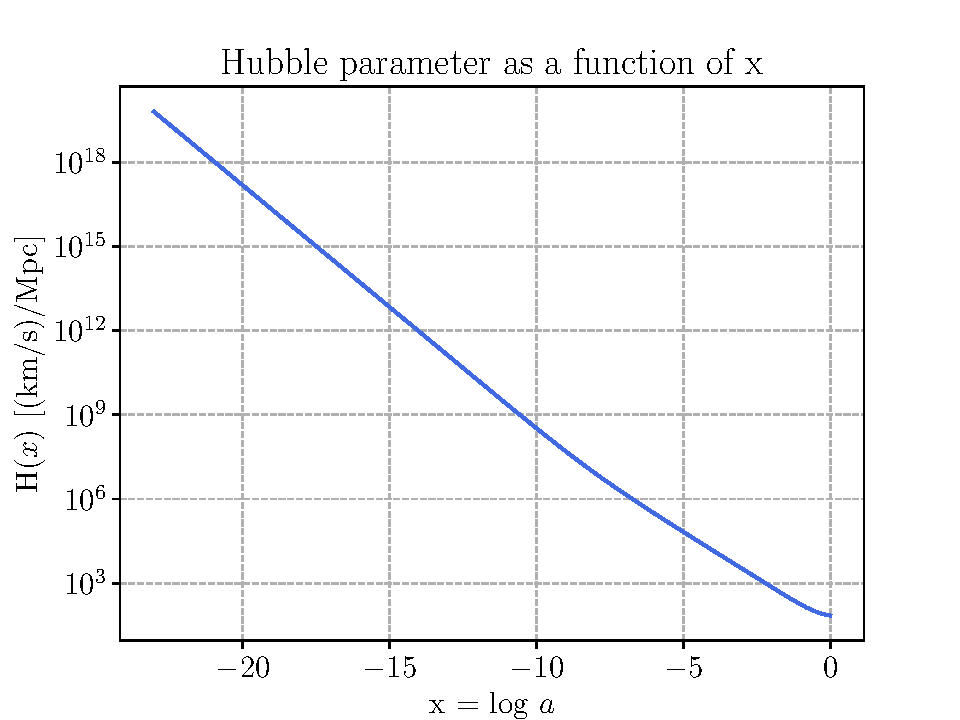
\includegraphics[width = 0.9\textwidth]{H_x.pdf}
    \caption{The evolution of the Hubble parameter as a function of
    $x$.}
    \label{fig: H_x}
\end{figure}

\begin{figure}
    \centering
    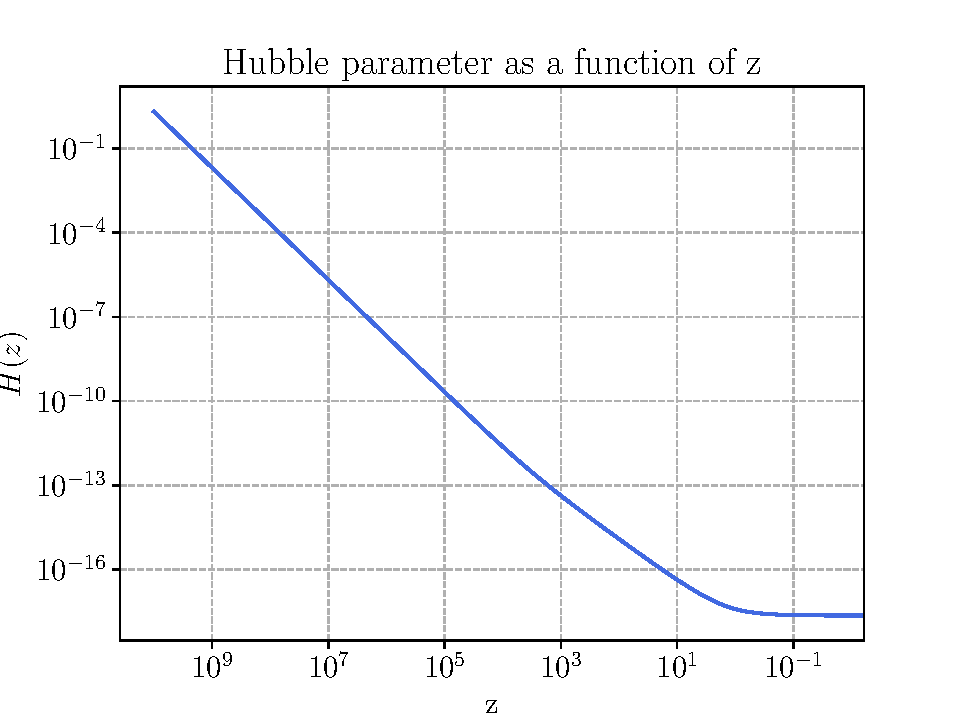
\includegraphics[width = 0.9\textwidth]{H_z.pdf}
    \caption{The evolution of the Hubble parameter as a function of
    $z$.}
    \label{fig: H_z}
\end{figure}

The calculated conformal time can be seen in figure \ref{fig: eta}
which also includes the splined data. The splined curve only resolves
the area of $x < 7$ as this seems to be the epoch where the conformal
time changes behaviour. This is likely connected to the fact that the
Universe goes from being radiation dominated to dark matter dominated.

\begin{figure}
    \centering
    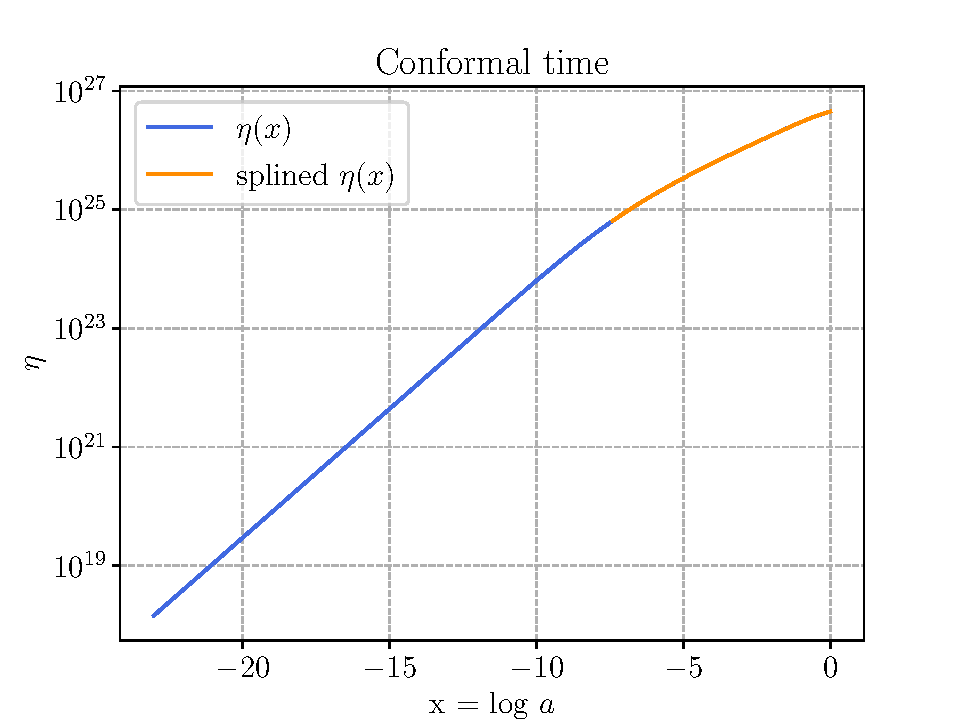
\includegraphics[width = 0.9\textwidth]{eta.pdf}
    \caption{The evolution of the conformal time, plotted together with
    the splined conformal time.}
    \label{fig: eta}
\end{figure}

\section{Conclusion}
We have calculated the expansion history of the universe in addition to
the studying the evolution of the background densities. All quantities
behave in an expected manner which suggest that our code is doing its
job correctly. We are therefore ready to apply our methods and results
to the coming milestone 2 where we are to study the recombination
history of the Universe.

\nocite{*}
\bibliography{references}{}
\bibliographystyle{plain}
\end{document}